%\chapter{Traditional Information Retrieval}

% START OF INTRODUCTION

\section{Traditional Information Retrieval} 
Information retrieval is the process of obtaining information resources which are  relevant to an information need of user from a collection. Early work on Information Retrieval with respect to natural language processing concentrated on tokenization and normalization of terms to match the variations in the queries, and it was proved to be successful. Ranking methods in traditional information retrieval systems broadly classified as set theoretic based models, algebraic models and probabilistic models.



% END OF INTRODUCTION


% START OF RANKING

\section{Ranking Methods} \label{Ranking Methods}

\begin{figure}[h]
\begin{center}
%\fbox{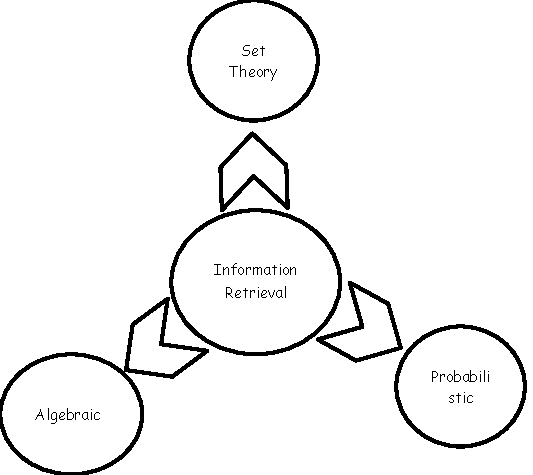
\includegraphics[scale=0.1,]{ir.pdf}}
\fbox{\scalebox{1}{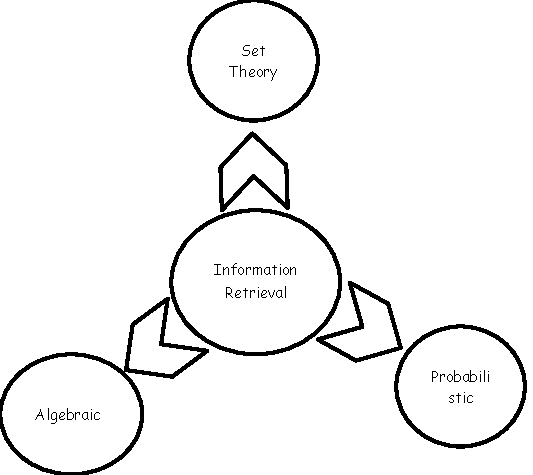
\includegraphics{ir.pdf}}}
\end{center}
\caption{Information Retrieval}
\end{figure}


% START OF SET

\subsection{Set theoretic models}
Set theoretic models represent documents and queries as sets of words. Similarities between documents and queries are calculated using set-theoretic operations such as union, intersection, difference on those sets.

\begin{enumerate}
\item{\textbf{Standard boolean model}}\\
Boolean Information Retrieval is based on Boolean logic and Set theory. The documents and user query are represented as set of terms. Retrieval is based on whether the documents have the query terms or not.\\
\textit{Query = ( \textit{india} AND NOT \textit{language} ) OR \textit{tamil}}\\
Resultant list of documents will have the word \textit{india} and not \textit{language} else the document should have word \textit{tamil} in it. This model has clean formalism, easy to implement but exact match results in either too many documents or too few documents, difficult to rank since the similarity measure is boolean and hard to frame query as boolean expression. 

\item{\textbf{Extended boolean model}}\\
In the above standard boolean model, all the query terms are considered with equal importance. However in reality, not all the query terms have equal importance in deciding relevance of document. Consider the query terms \textit{is} and \textit{algebra}, \textit{is} will appear in many of documents whereas \textit{algebra} will appear in a few of documents only. So \textit{algebra} must play more role in deciding the documents relevance. This model combines the characteristics of vector space model and standard boolean model then ranks the documents based on its similarity to query.\\
The weight of term $K_{x}$ in document $d_{j}$ is measured by its normalized term frequency
\begin{equation}
W_{x,j} =  f_{x,j} * \frac{Idf_{x}}{max_{i} Idf_{x}}
\end{equation}
where $Idf_{x}$ is inverse document frequency.
Consider a generalized conjunctive query,
\begin{equation}
Q_{or} = K_{1} \vee K_{2} \vee K_{3} .... \vee K_{t}
\end{equation}
The similarity between $Q_{or}$ and $d_{j}$ is defined as 
\begin{equation}
sim(Q_{or}, d_{j}) = \sqrt{\frac{w_{1}^{2} + w_{2}^{2} ...+w_{t}^{2}} {t}}
\end{equation}
Consider a generalized disjunctive query, 
\begin{equation}
Q_{and} = K_{1} \wedge K_{2}  \wedge  K_{3} ....  \wedge  K_{t} 
\end{equation}
The similarity between $Q_{or}$ and $d_{j}$ is defined as 
\begin{equation}
sim(Q_{and}, d_{j}) = \sqrt{\frac{(1-w_{1})^{2} + (1-w_{2})^{2} ...+(1-w_{2})^{2}} {t}}
\end{equation}

\item{\textbf{Fuzzy set retrieval}}\\
In fuzzy set theory, every element has a degree of membership to a given set instead of traditional membership(member or not). In information retrieval, each query term is considered as a fuzzy set and has varying degree of membership with each document depends on its relevance. To calculate semantic similarity between documents and a query, the query expression is modified to a set of conjunctive components. Each conjunctive component associates with a fuzzy set of documents and the union of the fuzzy sets are processed by Boolean operations. Finally, the membership value of each document in the processed fuzzy set is computed and ranked.

\end{enumerate}

% END OF SET

% START OF ALG MODEL

\subsection{Algebraic models}
Algebraic models represent documents and queries as vectors, matrices, or tuples. The similarity of the query vector and document vector is represented as a scalar value.

\begin{enumerate}
\item{\textbf{Vector space model}}\\
Vector space model is an Algebraic model which represents the documents as vectors of index terms. and Query also considered to be a vector of same dimentsion. Documents and queries are represented as vectors,
\begin{equation*}
\begin{split}
D_{j} = ( d_{1,j},d_{2,j},d_{3,j},,,,,d_{t,j}) & \\
Q = ( q_{1},q_{2},q_{3},,,,,q_{t} ) &
\end{split}
\end{equation*}
Each dimension of this vectors corresponds to one term in the vocabulary. If term occurs in the document or query, its value in the vector is non zero. Widely used method for computing the vector value is using the tf-idf wight calculation based on the terms frequency and inverse document frequency.  Term frequency is frequency of a term in a document, often normalized to document length to prevent biased ranking towards lengthy documents. Inverse document frequency is frequency of a term occurring document collection.

Document similarity is calculated by comparing the angle between each document vector and query vector. In practice cosine value of angle is used, 
\begin{equation}
cos(\theta) = \frac{D.Q}{||D||||Q||}
\end{equation}

\item{\textbf{Generalized vetor space model}}\\
Generalized vector space model is generalized version of the vector space model. GVSM is extended to avoid the issues that the orthogonality assumption of the vector space model creates. GVSM introduces term to term correlations $t_{i}.t_{j}$ .\\

\begin{equation}
sim(d_k, q) = \frac{ \sum_{j=1}^{n} \sum_{i=1}^{n} w_{i,k} * w_{j,q} * t_{i}.t_{j}  }{\sqrt{\sum_{i=1}^{n} w_{i,k}^2} * \sqrt{\sum_{i=1}^{n} w_{i,q}^2}}
\end{equation}
Term to term correlations are computed from using
\begin{enumerate}
\item{semantic correlations between terms using wordnet, ontology, \textit{etc}.}
\item{co-occurence statistics from large corpora.}
\end{enumerate}

\item{\textbf{Latent semantic analysis}}\\
Latent semantic analysis is a technique of analyzing relationships between a set of documents and a term. And this is done by producing set of latent concepts related to document and terms. LSA assumes that words which have close semantics will co-occur. A term-document matrix constructed by filling each cell with frequency of term in each document. Once term-document is constructed, single valued decomposition is used to split term-document matrix into three parts. Applying rank reduction to this matrix, ensures that terms, document which have similar move together like clustering. This decomposed matrices can be used to find relevance between term-term, document-term and document-document.


\end{enumerate}

% END OF ALG MODEL

% START OF PROB MODEL

\subsection {Probabilistic models}

Probabilistic models treat the process of document retrieval as a probabilistic inference. Similarities are computed as probabilities that a document is relevant for a given query. These models includes Binary Independent model (BIM), Okapi BM25, BM25F, Language Model and KL divergence. %and Latent Drichlet Allocation (LDA). 
\begin{enumerate}
\item{\textbf{Binary Independence model}}\\
Binary Independece Model (BIM) considers the documents as binary vectors. Each vector dimension marks the presence or absence of term in a document. Terms are independently distributed in relevant documents and same for irrelevant documents.
\begin{equation}
P(R|x,q) = \frac{P(x|R,q) P(R|q)}{P(x|q)}
\end{equation}
where $P(x|R=1,q)$ and $P(x|R=0,q)$ are the probabilities of retrieving a relevant or irrelevant document. 

\item{\textbf{Language Models}}\\
With query Q as input, retrieved documents are ranked based on the probability that the documents language model can generate the terms of the query, $P(Q|D_k)$. The method to use language models in information retrieval is the query likelihood model.
\begin{equation}
P(D/Q) = P(Q/D) P(D) / P(Q) 
\end{equation}
P(Q) is same for all documents so it can be ignored. The prior probability of a document P(D) is often treated as uniform across all documents, so it can also be ignored. With these simplifications, documents are ranked by P(Q/D).
\begin{equation}
P(Q/D) = K_q \prod_{t \in V}{ P(t/D)^{tf_{t,d}}}
\end{equation}
%\item{\textbf{Latent Drichlet Allocation}}\\
%In Latent Drichlet Allocation, 
%\item{\textbf{probabilisitc Latent semantic indexing}}\\
\item{\textbf{KL divergence}}\\
Kullback-Leibler divergence measures the divergence between two probability distributions. If query and documents are represented as probability distributions, then using KL divergence the dissimilarity can be calculated. 
\begin{equation}
\begin{split}
sim(D,Q) = - D (D,Q) &= - \sum_w p(w|Q) \frac{log p(w|Q)}{log p(w|D)} \\
		  			 &= - \sum_w p(w|Q) log p(w|Q) + (- \sum_w p(w|Q) log p(w|D))\\
\end{split}		 
\end{equation}

\end{enumerate}


% END OF PROB MODEL
% END OF RANKING


% START OF ISSUES

\section {Limitations} 

Information retrieval systems are encountering difficulties by their limited understanding of 
\begin{enumerate}
\item{user queries}
\item{the content of the Web}
\end{enumerate}
So, they are limited in their ways of matching the two. In face of ambiguity in understanding the meaning of information need, current retrieval systems manage to mask their confusion, by 

\begin{enumerate}
\item{explicitly introducing diversity to results (letting the user choose)}
\item{relying on some notion of popularity, hoping that the user will be interested in the most common interpretation of the query}
\end{enumerate}

% END OF ISSUES

